\subsection{Descripción:}

En este ejercicio debemos encontrar el costo mínimo de un conjunto de impresiones, dado un grupo de trabajos.\\

Para realizar la impresión contamos con dos máquinas iguales donde podemos repartir los trabajos, estos tienen un costo particular según quién fué el trabajo previo o si son el primer trabajo de la máquina.\\
Además se debe cumplir un orden en las impresiones, el trabajo i no puede ir antes que el j si i>j.\\
Es decir, los trabajos se pueden repartir entre las máquinas de muchas maneras distintas, pero para calcular el costo debe tenerse en cuenta el orden mencionado anteriormente.\\

Es nuestra meta encontrar la forma de repartirlos que abarate el costo total de las impresiones.\\

Por ejemplo si contamos con estos trabajos i, con sus respectivos precios respecto al trabajo anterior j:\\
\begin{center}
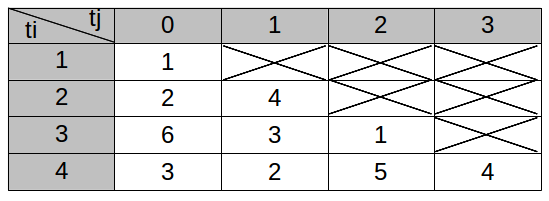
\includegraphics[scale=0.7]{ej1/descripcion1.png} \\
\end{center}

Entonces la solución con costo mínimo sería:\\
\begin{center}
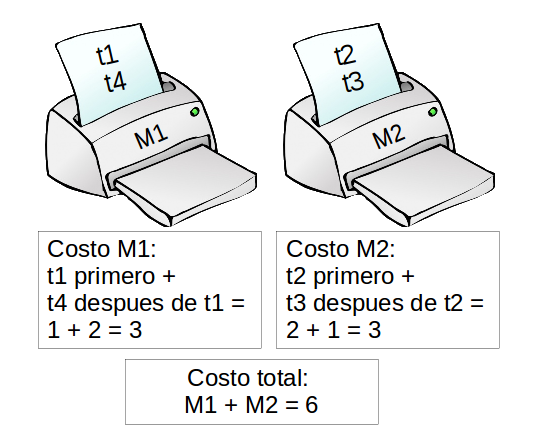
\includegraphics[scale=0.6]{ej1/descripcion2.png}\\
\end{center}



